\documentclass[11pt]{report}
\usepackage{graphicx}
\usepackage{parskip}
\usepackage{mathtools}

\title{Pursuit Curves}
\author{David Grant}
\date{June 2015}

\begin{document}

\maketitle

\section*{1.}

\begin{center}
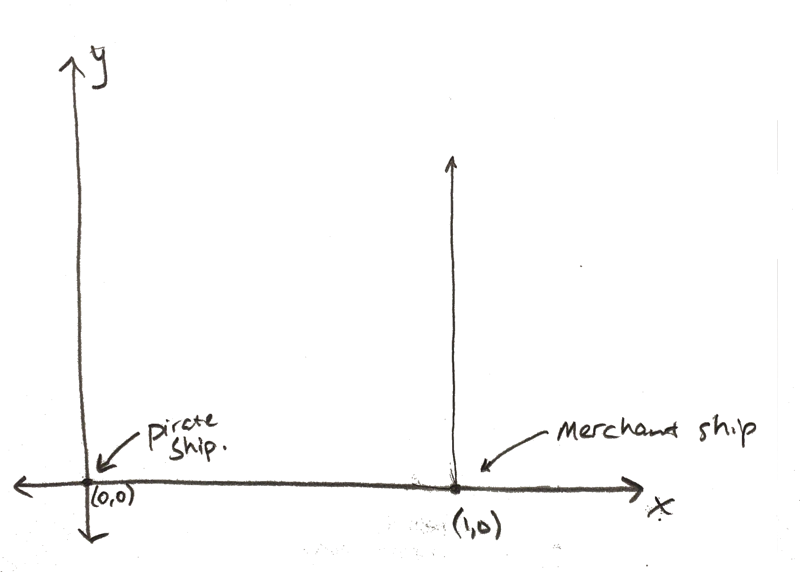
\includegraphics[width=\linewidth]{sketch1}
\textit{Sketch of initial ship position and trajectory of
merchant ship.} 
\end{center}

\section*{2.}

Since both ships begin at the same $y$ coordinate and the merchant
ship is constantly traveling due north, it makes sense that the pirate ship's path will be a non-linear, square-looking one.

\section*{3.}

The merchant ship will have traveled $V_{m}t$ ...\textit{units}... after $t$ hours. At this time, the merchant ship's coordinates will be $(1, V_{m}t)$.

\section*{4.}

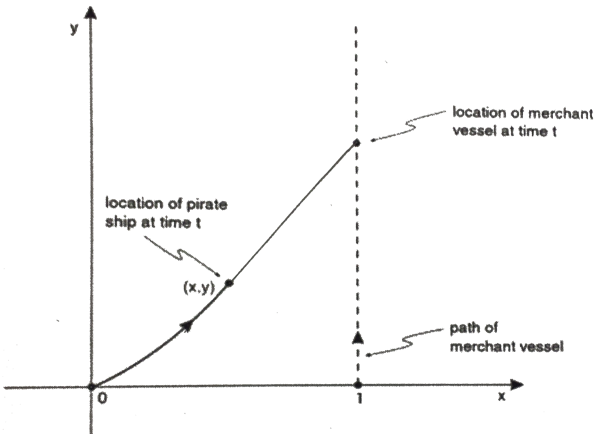
\includegraphics[width=\linewidth]{part4}

\section*{5.}

The slope of this tangent line between the pirate and merchant ships is:

$$
	\frac{y_{p} - y_{m}} {x_{p} - x_{m}}
	\rightarrow
	\frac{y_{p} - V_{m}t} {x_{p} - 1}
$$

This is the instantaneous slope of the pirate ship, so:

$$
    \frac{dy}{dx} = \frac{y_{p} - V_{m}t} {x_{p} - 1}
$$

Solving for $t$:

$$ \frac{dy}{dx}(x_p - 1) = y_p - V_mt $$
$$ \frac{dy}{dx}(x_p - 1) - y_p = -V_mt $$
$$ \frac
	{\frac{dy}{dx}(x_p - 1) - y_p}
	{-V_m}
   = t $$
   
$$ t = \frac
	{-\frac{dy}{dx}(x_p - 1) + y_p}
	{V_m}
$$



\section*{6.}

We're given this equality, which makes enough sense:

$$ V_pt = \int_0^x \sqrt{1 + \Big(\frac{dy}{dz}\Big)^2} dz $$

Solving for $t$:

$$ t = \frac{1}{V_p} \int_0^x \sqrt{1 + \Big(\frac{dy}{dz}\Big)^2} dz $$

\section*{7.}

\begin{quote}
	Using the results from \#5 and \#6 as well as letting
	$p(x) = \frac{dy}{dx}$, show that
	$
	\frac{1}{V_p} \int_0^x \sqrt{1 + p^2(z)} dz
	=
	\frac{y}{V_m}
	- \frac {(x-1)} {V_m} \cdot p(x)$.
\end{quote}

First, we define $p$:
$$p(x) = \frac{dy}{dx}$$
Our conclusion from \#6:
$$ t = \frac{1}{V_p} \int_0^x \sqrt{1 + \Big(\frac{dy}{dz}\Big)^2} dz $$
becomes
$$ t = \frac{1}{V_p} \int_0^x \sqrt{1 + p^2(z)} dz $$

Recalling our conclusion from \#5:
$$ t = \frac
	{-\frac{dy}{dx}(x_p - 1) + y_p}
	{V_m}
$$

This can be reorganized to:
$$ t = \frac{-p(x)(x - 1)}{V_m}
	+
	\frac{y}{V_m}
$$
$$ t = p(x) \cdot \frac{-(x - 1)}{V_m}
	+
	\frac{y}{V_m}
$$
$$ t = \frac{y}{V_m} -  \frac {(x - 1)}{V_m} \cdot p(x) $$

So,
$$
\frac{1}{V_p} \int_0^x \sqrt{1 + p^2(z)} dz
=
\frac{y}{V_m} -  \frac{(x - 1)}{V_m} \cdot p(x)
$$

\section*{8.}

\begin{quote}
	Using some ideas from the FTC, take a derivative in terms of $x$ on both sides of the equation in \#7 [...].
\end{quote}


\textbf{Left-hand side:}

$$
\frac{d}{dx}\Big(\frac{1}{V_p} \int_0^x \sqrt{1 + p^2(z)} dz\Big)
\rightarrow
\frac{1}{V_p} \cdot \frac{d}{dx}\Big(\int_0^x \sqrt{1 + p^2(z)} dz\Big)
$$

Applying FTC$_2$ our LHS becomes:

$$
\frac{1}{V_p} \cdot \sqrt{1 + p^2(x)}
$$

\textbf{Now, the RHS:}

$$
\frac{d}{dx}
\Big(
\frac{y}{V_m} -  \frac{x-1}{V_m} \cdot p(x)
\Big)
$$

$$
\frac{1}{V_m}
\Biggr(
	\frac{dy}{dx}
	-
	\frac{d}{dx}
	\Big(
	(x - 1) \cdot p(x)
	\Big)
\Biggr)
$$

$$
\frac{1}{V_m}
\Biggr(
	\frac{dy}{dx}
	-
	\Big(
	p(x) + (x-1) \cdot p'(x)
	\Big)
\Biggr)
\rightarrow
\frac{1}{V_m}
\Biggr(
	\frac{dy}{dx}
	-
	\Big(
	\frac{dy}{dx} + (x-1) \cdot \frac{dp}{dx}
	\Big)
\Biggr)
$$

$$
\frac{1}{V_m}
\Big(
	-
	(x-1) \cdot \frac{dp}{dx}
\Big)
$$

$$
-\frac{(x-1)}{V_m}
\cdot \frac{dp}{dx}
$$

Since we've just taken the derivative of both sides, they're still equal, and
we get the desired equality:

$$
\frac{1}{V_p} \sqrt{1 + p^2(x)}
=
-\frac{(x-1)}{V_m} \frac{dp}{dx}
$$

Simplify this further by multiplying both sides by $-V_m$.

$$
(-V_m)
\frac{1}{V_p} \sqrt{1 + p^2(x)}
=
(-V_m)
\frac{-(x-1)}{V_m} \frac{dp}{dx}
$$

$$
\frac{-V_m}{V_p} \sqrt{1 + p^2(x)}
=
(x-1) \frac{dp}{dx}
$$

...and let $n = \frac{Vm}{Vp}$, the ratio of the
merchant ship's velocity to the pirate ship's velocity.

$$
-n \sqrt{1 + p^2(x)}
=
(x-1) \frac{dp}{dx}
$$

\begin{description}

	\item[When $n > 1$], the merchant ship is moving faster than the pirate ship.
	\item[When $n = 1$], the ships are traveling at the same velocity.
	\item[When $n < 1$], the pirate ship is moving faster than the
merchant ship.
\end{description}

The case when $n < 1$ is the most important to us, because the pirates will potentially be closing in on the merchants.

(Note that since the merchant ship is traveling in a "bee" line and the pirate ship is 
following some curve, the ratio $n$ will have to be some amount \emph{under} $1$ in order
for the pirate ship to actually get closer to the merchant ship.)

\section*{9.}

We now have a differential equation that looks like:

$$
(x-1) \frac{dp}{dx}
=
-n \sqrt{1 + p^2(x)}
$$

We use separation of variables to take the integrals:

$$
\int \frac{1}{\sqrt{1 + p^2(x)}} dp
=
\int \frac{-n}{x-1} dx
$$

For the LHS, my computer gives me:

$$
\int \frac{1}{\sqrt{1 + p^2(x)}} dp
=
sinh^{-1}(p) + C
$$

Per the definition of $sinh^{-1}$:

$$
sinh^{-1}(p) = ln(p + \sqrt{p^2 + 1})
$$

For the RHS:

$$
\int \frac{-n}{x-1} dx
\rightarrow
n \cdot \int \frac{1}{1-x} dx
$$

$$ = -n \cdot ln(1-x) + C $$

Altogether:

$$
ln(p + \sqrt{p^2 + 1}) + C
=
-n \cdot ln(1-x)
$$

\section*{10.}

When $t=0$, $x$ is also $0$. At this time, the instantaneous value of $p$, which was
defined as $\frac{dy}{dx}$, will be $\frac{0}{something}$. That is, at this time
the pirate ship will be proceeding due west directly at the merchant ship.
$p_x$ will be changing and $p_y$ will not.

Recalling our previous equation:
$$
ln(p + \sqrt{p^2 + 1}) + C
=
-n \cdot ln(1-x)
$$
We can plug in some values since we know that when $x=0$, $p$ is also $0$:
$$
ln(0 + \sqrt{0^2 + 1}) + C
=
-n \cdot ln(1-0)
$$
$$ ln(1) + C = -n \cdot ln(1) $$
$$ C = 0 $$

\section*{11.}

Rearranging using various natural log rules:

$$ ln(p + \sqrt{p^2 + 1}) = -n \cdot ln(1-x) $$
$$ ln(p + \sqrt{p^2 + 1}) = -ln((1-x)^n) $$
$$ ln(p + \sqrt{p^2 + 1}) + ln((1-x)^n) = 0 $$
$$ ln\Big((p + \sqrt{p^2 + 1}) (1-x)^n \Big) = 0 $$
$$ e^{ln((p + \sqrt{p^2 + 1}) (1-x)^n )} = e^0 $$
$$(p + \sqrt{p^2 + 1}) (1-x)^n = 1$$

\section*{12.}

Letting $q=(1-x)^{-n}$:

$$(p + \sqrt{p^2 + 1}) \frac{1}{q} = 1$$
$$p + \sqrt{p^2 + 1} = q$$
$$\sqrt{p^2 + 1} = q - p$$
$$p^2 + 1 = (q - p)^2$$
$$p^2 + 1 = q^2 + p^2 - 2qp$$
$$p^2 - p^2 = q^2 - 2qp - 1$$
$$2qp = q^2 - 1$$
$$p = \frac{q^2 - 1}{2q}$$

$$p = \frac{1}{2}(q - \frac{1}{q})$$


\end{document}
